\section{Paradigme de l'Induction}
\subsection{Qu'est-ce que l'Induction ?}
\noindent Supposons un chat et un cheval. Ces deux entités se distinguent de part leur silhouette, leur dimension, leur vitesse de déplacement etc... Il est aisé de discriminer ces deux animaux et ce, sans erreur notable. Cependant, l'observateur n'a jamais pu observer \textit{l'intégralité} des spécimens de chats et de chevaux. A partir d'un volume limité d'observations, il a appris à \textit{discriminer}, i.e isoler des caractéristiques permettant  de réaliser une identification. Ce comportement est appelé \textbf{induction} ou encore \textbf{généralisation}.\\

\noindent \textbf{Remarque}: Le paragraphe ci-dessus illustre un cas d'\textit{induction} implicite. En effet, dire que "\textit{tout le monde peut discriminer...}" est une \textit{généralisation}. Afin d'être rigoureux, il aurait fallu indiquer l'environnement où cette affirmation se vérifie (pays, régions, aptitudes de l'observateur...). Et même dans cette situation, le phénomène de \textit{généralisation} est encore présent. En réalité, la seule affirmation véritablement valide serait comparable à "\textit{La quasi-totalité des individus observés \textbf{respectant des conditions spécifiques} sont capables de réaliser cette discrimination}". La notion de \textit{conditions} est primordiale car elle détermine les spécificités de l'environnement. Pour illustrer, il est évident qu'un individu valide et un aveugle réalisent une discrimination de ce phénomène de manière distincte.\\

\noindent L'objectif de l'\textbf{induction artificielle} est de déterminer un ensemble de  \textit{règles de décision} de manière \textit{automatique} à partir d'un échantillon limité de données illustrant le phénomène étudié. Cette ensemble de règles peut avoir deux objectifs (non exclusifs):
\begin{itemize}
    \item \textbf{Réaliser une prédiction} sur une observation spécifique. Par exemple, "Cette image représente un chat ou un chien ?".

    \item \textbf{Extraire une théorie du phénomène observé}. En d'autres mots, être capable de faire une prédiction et d'expliquer le phénomène. Par exemple, "Cet animal est un chat car il chasse une souris".
\end{itemize}

\noindent Trois questions fondamentales constituent la problèmatique de l'induction:
\begin{itemize}
    \item Ais-je le droit de généraliser à partir d'un échantillon fini de donné ?
    \item Comment réaliser l'extrapolation ? Comment savoir si comprendre les données disponibles permettra une bonne compréhension du phénomène durant la phase de prédiction ?
    \item Quelle garantie peut-on avoir sur l'extrapolation réalisée ?
\end{itemize}

\subsection{Les différentes formes d'apprentissage}

\noindent L'apprentissage peut se présenter sous différentes formes. Le type d'apprentissage dépend de la \textbf{tâche} à accomplir mais surtout du \textbf{type} et du \textbf{volume} de données disponibles. La donnée est au coeur de l'apprentissage et sa qualité est \textbf{primordiale}\footnote{Définir ce qu'est une donnée \textit{qualitative} peut être ardue.}. L'hégémonie des entreprises chinoises et américaines dans le domaine de l'intelligence artificielle\footnote{Et plus globalement, de la Donnée} repose en partie sur le volume de données qu'ils ont emmagasiné\footnote{Au détriment, parfois, de la vie privée...} au fil des années. Peu importe l'efficacité d'un algorithme d'apprentissage, si la donnée d'apprentissage est mauvaise alors la qualité de la prédiction le sera aussi !\\

\noindent Il existe de nombreuses formes d'apprentissage. Néanmoins, plusieurs méthodes sortent du lot du fait de leur maturité et surtout, de leur efficacité.

\subsubsection{Apprentissage supervisé}

\noindent L'apprentissage supervisé est la méthode d'apprentissage la plus populaire actuellement. La majorité des approches de \textbf{Deep Learning} reposent sur ce type d'apprentissage bien qu'elles tendent à se diversifier de plus en plus avec les avancées de la Recherche.\\

\noindent L'apprentissage supervisé permet un apprentissage à partir d'exemples dits \textbf{labellisés}. Une donnée labellisée se présente sous la forme d'un couple:
$$\mathcal{X} \rightarrow \mathcal{Y}: \ (x_i,y_i)_{i \in \mathbb{N}}$$

\noindent $\mathcal{X}$ désigne une distribution qui illustre un phénomène à observer et à discriminer. Par exemple, $\mathcal{X}$ peut être associée à une distribution sur $\mathbb{R}^{784}$  si le phénomène à observer est caractérisé par des images (plus spécifiquement, des pixels) de chats de 784 pixels. $\mathcal{Y}$ correspond à l'espace de prédiction. Ainsi, supposons une prédiction binaire est/n'est pas, alors $\mathcal{Y}=[0,1]$.\\

\noindent Un ensemble d'apprentissage, dans le cadre supervisé, est un ensemble de données labellisées. Le volume de données nécessaires est difficile à déterminer. Néanmoins, la quantité est très importante et proportionnelle à la complexité de l'algorithme d'apprentissage et de la tâche à apprendre. Le manque de données disponibles est une des raisons du retard des pays européens du fait d'une politique sur les libertés individuelles (vie privée) plus restrictive.\\

\noindent L'objectif de l'apprentissage supervisé est de définir une fonction f (nommé \textit{superviseur}) telle que $f(x)=y$ pour $(x,y) \in \mathcal{X} \times \mathcal{Y}$. Il est important de considérer qu'un ensemble d'apprentissage n'illustre pas l'intégralité d'un phénomène mais uniquement une partie. La capacité de généralisation de f sur l'ensemble des cas observables (y compris ceux non représentés dans l'ensemble d'apprentissage) définit la qualité de la prédiction de l'algorithme. Ainsi le \textit{superviseur} apprend à isoler des \textit{règles} (ou des caractéristiques) qui discriminent chacune des classes représentées par l'ensemble d'apprentissage et supposant qu'elles se généralisent sur l'ensemble du phénomène. Il est donc fondamental que l'ensemble d'apprentissage soit représentatif du phénomène considéré. \\

\noindent Dans le cadre de l'apprentissage supervisé, nous pouvons définir \textbf{trois} problèmes-types:
\begin{itemize}
    \item \textbf{Classification}: Une \textit{classification} est définie lorsque $\mathcal{Y}={1,...,N}$, i.e $\mathcal{Y}$ est un espace discret (et fini). Un problème de classification revient donc à étiqueter une entrée inconnue avec un label. Nous pouvons citer, par exemple, la discrimination d'images selon ce qu'elles représentent. Une classification peut être \textit{binaire}. Nous avons donc un problème de type "est/n'est pas" ($|\mathcal{Y}|=2$). Au contraire, une classification peut être \textit{multi-classe}. De ce fait, elle ne cherche plus à discriminer deux classes mais n classes distinctes ($|\mathcal{Y}|=N$).

    \item \textbf{Régression}: Une \textit{régression} est définie lorsque $\mathcal{Y} \in \mathbb{R}$, i.e $\mathcal{Y}$ est continue. Une régression consiste donc à prédire une valeur. L'exemple standard de régression est la prédiction de prix ou d'une valeur dimensionnelle quelconque.

    \item \textbf{Prédiction structurée}: $\mathcal{Y}$ peut être associée à une \textit{structure}, i.e une entité dite complexe qui se présente souvent sous forme de \textit{graphes}. Ce type de prédiction est très employé dans le secteur médical, notamment pour les problématiques associées à l'étude génétique.
\end{itemize}

\subsubsection{Apprentissage non supervisé}

\noindent L'apprentissage \textit{non-supervisé} est caractérisé par l'exploitation de données \textbf{non labellisées}, i.e de la forme $\mathcal{X}: \ x_{i \in \mathbb{R}}$.\\

\noindent Comme les données ne sont pas catégorisées, il n'est pas possible d'apprendre une fonction d'association entre les données observées d'un phénomène et un étiquetage quelconque. L'objectif est donc d'exploiter les similarités entre les données afin de pouvoir les regrouper par groupes d'entités similaires appelés \textit{cluster}. \\

\noindent Ce type d'approche est très populaire car elle répond à deux problématiques industrielles très importantes:
\begin{itemize}
    \item \textbf{Difficulté de la labellisation}: Labelliser des données peut être difficile et/ou coûteux en ressources (temporelles et financières). En s'émancipant de la labellisation, de fortes économies sont réalisées.

    \item \textbf{Découverte de phénomène}: L'apprentissage supervisé suppose une connaissance du phénomène à discriminer. En effet, labelliser une donnée nécessite de connaître ce qu'elle représente. Cette condition de \textit{supervision} est très problématique lorsque le phénomène observé est inconnu (ou encore partiellement connu). Au contraire, l'apprentissage non supervisé, en ignorant la condition de supervision, s'émancipe de l'obligation de connaissance du phénomène. Cette approche est donc capable d'apprendre un phénomène inconnu et de ce fait, en découvrir de nouveaux et les expliciter. \\

    \noindent Cette qualité est une plus-value au niveau industriel car elle permet de détecter les tendances  et l'évolution des comportements. Elle est, par exemple, très exploitée dans le cadre de l'analyse comportementale des utilisateurs, des tendances de consommation etc...

    \item \textbf{Nombre de classes variable}: L'apprentissage supervisé nécessite un nombre de classes fini et constant. Au contraire, l'apprentissage non supervisé permet une prédiction indépendante d'une condition préalable sur les classes.
\end{itemize}

\noindent L'apprentissage supervisé apprend des règles durant son apprentissage qui lui permettra de discriminer une donnée inconnue. Au contraire, l'apprentissage non supervisé n'est pas capable de définir une classe par discrimination. En effet, l'apprentissage non supervisé apprend à détecter les similarités entre les données. De ce fait, il n'est pas capable de discriminer une classe car il n'a pas conscience des règles qui la constitue ni même de son existence. Cette émancipation d'une connaissance \textit{a priori} des classes permet une plus grande souplesse d'utilisation mais aussi une impossibilité de catégorisation. L'apprentissage non supervisé repose sur l'idée que deux données similaires sont associées à une même catégorie. Ainsi, il est possible de définir des groupements de données présentant un comportement similaire mais à la labellisation inconnue. La différence entre les deux méthodes d'apprentissage est représentée sur la Figure \ref{super_unsuper}.\\

\begin{figure}
    \centering
    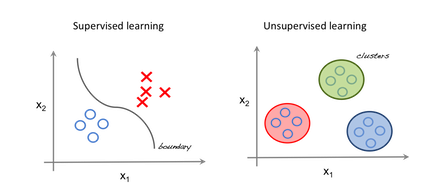
\includegraphics[scale=0.5]{./tex/induction/unsuper.png}
    \caption{Différence entre apprentissage supervisé en non supervisé}
    \label{super_unsuper}
\end{figure}


\subsubsection{Apprentissage semi-supervisé}

\noindent Une approche alternative, nommée \textit{apprentissage semi-supervisé}, propose d'exploiter des données \textbf{labellisées} et \textbf{non labellisées}. Elle est donc comparable à un mélange entre apprentissage \textit{supervisé} et \textit{non supervisé}. \\

\noindent Cette forme d'apprentissage cherche à combiner les avantages des deux approches tout en corrigeant mutuellement leurs défauts propres. L'objectif principal de cette méthode d'apprentissage est de limiter le volume de données labellisées nécessaires à l'apprentissage supervisé en reposant sur la capacité d'association des données que procure l'apprentissage non supervisé. Ainsi, à partir d'un volume restreint de données labellisées, l'algorithme sera capable d'améliorer ses règles de discrimination à partir de données non labellisées grâce aux capacités non supervisées de l'algorithme.\\

\noindent Les approches standards semi-supervisées sont l'\textit{auto-apprentissage} et le \textit{co-apprentissage}.\\

\noindent L'\textit{auto-apprentissage} cherche à apprendre un superviseur à partir d'un volume restreint de données. Le superviseur discrimine alors des données non labellisées et les prédictions à forte confiance sont ajoutées à l'ensemble d'apprentissage. Un nouveau apprentissage est alors de nouveau réalisé avec le nouveau ensemble d'apprentissage. Ce cycle peut être répété plusieurs fois.\\

\noindent Le \textit{co-apprentissage} part du postulat qu'il existe 2 (ou plus) projections indépendantes d'un même espace de données. Ainsi, il va apprendre un classifieur sur chacune de ces projections et réaliser des prédictions indépendantes. Si la prédiction des classifieurs pour une même donnée est identique\footnote{Au moins, à la majorité...}, alors la donnée est discriminée par la classe prédite.\\

\noindent Par exemple, supposons que nous voulons discriminer un individu selon son sexe. La taille, le poids et la pilosité sont des critères discriminants. Ainsi, trois projections selon ces variables permettent la création de trois classifieurs qui évalueront un individu selon ces trois critères. Dans les faits, la taille et les poids ne sont pas complètement indépendants\footnote{Le poids et la taille sont corrélés entre eux.}. Néanmoins, on peut faire l'hypothèse qu'ils le sont.

\subsubsection{Apprentissage par transfert}
\noindent L'apprentissage automatique est une tâche coûteuse en ressources et en temps. De même, elle nécessite un important volume de données. Ces contraintes sont déterminantes pour le développement et l'exploitation de l'intelligence artificielle. En effet, il peut être difficile d'avoir des données associées à une tâche précise, de même qu'il n'est pas toujours possible d'avoir à disposition, une forte capacité de calculs (ou de temps).\\

\noindent C'est dans cet environnement que l'apprentissage par transfert (\textit{Transfer Learning}) prend toute son importance. En effet, ce paradigme repose sur l'idée que les connaissances acquises lors d'un apprentissage dans un environnement particulier peuvent être utilisées pour améliorer l'apprentissage dans un autre environnement. Ainsi, il n'est plus nécessaire de supposer un contexte strictement inconnu mais au contraire, en supposer une partie déjà définie. Cette approche permet donc un gain de temps d'apprentissage et une optimisation des données considérables, ce qui est critique pour l'industrie moderne.\\

\noindent Il ne s'agit pas d'une méthode d'apprentissage à proprement parler (comme l'apprentissage supervisé ou non supervisé) mais plutôt d'une optimisation de ces dernières. Elles sont donc complémentaires. Par exemple, dans le cadre de l'apprentissage supervisé, l'apprentissage par transfert implique la possibilité de réutiliser la connaissance de la structure de dépendance entre les caractéristiques et les étiquettes apprises dans un contexte afin d'améliorer l'inférence de la structure de dépendance dans un autre contexte.\\

\noindent Supposons un phénomène particulier (ou domaine) défini sur un espace $\mathcal{X}$ par une distribution $\mathcal{P}$. Nous avons donc un domaine $\mathcal{D}$ tel que $\mathcal{D}=(\mathcal{X}, \mathcal{P})$. Nous souhaitons réaliser une tâche $\mathcal{T}$ tel que $\mathcal{T}=(\mathcal{Y},f)$ avec f, fonction-cible définie telle que $f:\mathcal{X} \rightarrow \mathcal{Y}$.\\

\noindent Supposons un cas où nous disposons de deux domaines distincts avec une tâche définie par domaine. Le premier est le domaine-source $\mathcal{D}_S$ et possède une tâche $\mathcal{T}_S$. Le second est le domaine-cible et est défini par $\mathcal{D}_C$ et $\mathcal{T}_C$. L'objectif de l'apprentissage par transfert est d'améliorer l'apprentissage de $f_{\mathcal{T}_C}$ en utilisant la connaissance issue de $\mathcal{T}_S$, $\mathcal{D}_S$ en plus de $\mathcal{D}_C$, $\mathcal{T}_C$ avec des conditions d'inégalité entre les domaines et les tâches. Par exemple, $\mathcal{D}_S \neq \mathcal{D}_C$ et $\mathcal{T}_S \neq \mathcal{T}_C$. \\

\noindent Il existe trois grandes approches d'apprentissage par transfert (voir Figure \ref{transfer_l_pic}) :
\begin{enumerate}
    \item \textbf{Transductive}: Les deux domaines sont différents\footnote{Différents mais liés par un lien quelconque permettant le transfert !} mais la tâche est la même. De plus, nous ne possédons pas de label pour les données du domaine-cible. Nous avons donc:  $\mathcal{T}_S = \mathcal{T}_C$, $\mathcal{D}_S \neq \mathcal{D}_C$ et $\mathcal{D_{C|Y}}= \emptyset$. Le cas particulier où $\mathcal{D}_S = \mathcal{D}_C$ est néanmoins possible et exploite d'autres méthodes pour être exploitées. \\

    \item \textbf{Inductive}: Les deux domaines sont identiques mais les tâches diffèrent. Nous possédons les labels pour les deux domaines ou uniquement pour le domaine cible. Nous avons donc: $\mathcal{T}_S \neq \mathcal{T}_C$, $\mathcal{D}_S = \mathcal{D}_C$\\

    \item \textbf{Non-supervisée}: Les deux domaines sont différents et les tâches diffèrent aussi. Nous ne possédons pas les labels pour les deux domaines. Nous avons donc: $\mathcal{T}_S \neq \mathcal{T}_C$, $\mathcal{D}_S = \mathcal{D}_C$ et $\mathcal{D_{S|Y}} \neq \mathcal{D_{C|Y}}=\emptyset$.\\
\end{enumerate}

\begin{figure}
    \centering
    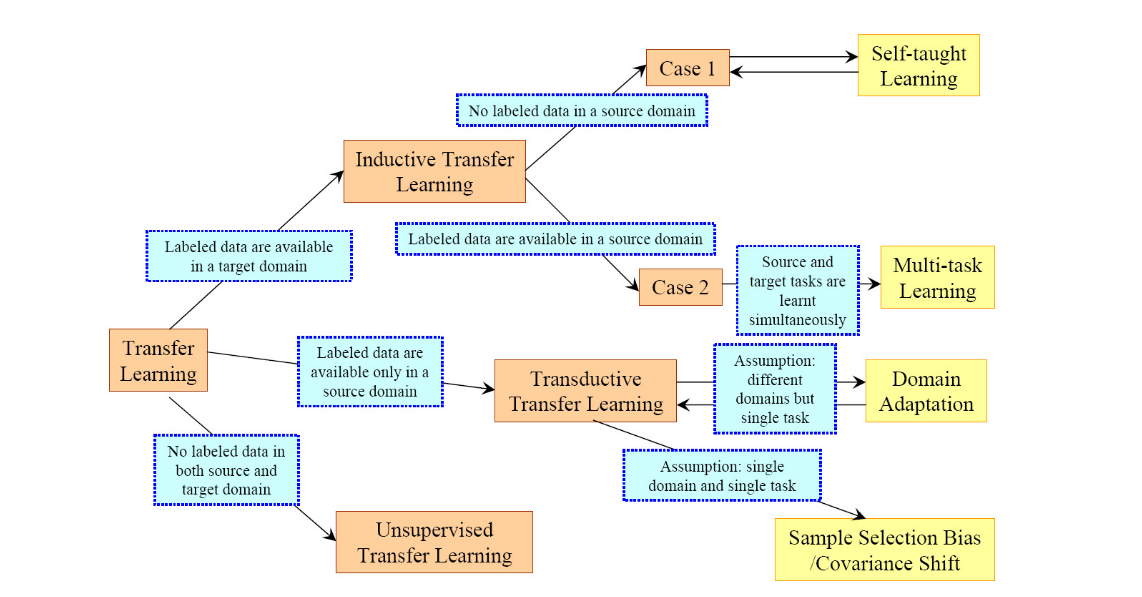
\includegraphics[scale=0.3]{./tex/induction/transfer_l.png}
    \caption{Les différentes approches d'apprentissage par transfert}
    \label{transfer_l_pic}
\end{figure}

\noindent De même, deux spécificités sont associées aux espaces des domaines. Ainsi, nous parlons d'apprentissage par transfert \textbf{homogène} si $\mathcal{X}_S=\mathcal{X}_C$. La différence se situe donc au niveau de la loi de probabilité associée à chacun des domaines. Si $\mathcal{X}_S \neq \mathcal{X}_C$, nous parlerons d'apprentissage par transfert \textbf{hétérogène}.\\

\noindent Quatre configurations de ces approches sont proposées: \textbf{Instance  Transfer}, \textbf{Feature Representation Transfer}, \textbf{Parameter Transfer} et \textbf{Relational Knowledge Transfer}\cite{transfer_l}.

\paragraph{Instance Transfer}

\noindent L'approche \textit{Instance Transfer} repose sur l'idée que des données issues du domaine source peuvent être utilisées dans un autre domaine (lié) à travers différentes méthodes de \textit{sampling} et de pondération.

\paragraph{Feature Representation Transfer}

\noindent L'approche \textit{Feature Representation Transfer} cherche à projeter la donnée issue du domaine-source dans un espace spécifique afin de faciliter la discrimination de $f_C$. Ainsi, nous définissons une fonction de projection $\phi: \mathcal{X} \rightarrow \mathcal{Z}$. De même, nous redéfinissons $h_C$ tel que $h_C=f(\phi(x);\theta_C)$.\\

\noindent Cette approche est exploitée pour modifier la donnée-source afin de faciliter l'apprentissage du modèle. Par exemple, si la donnée-source possède une dimension trop élevée, il peut être utile de la représenter à travers une dimension plus faible, ce qui permet de faciliter son apprentissage. Néanmoins, il est important de considérer la perte d'informations associée à une projection dans un autre espace.

\paragraph{Parameter Transfer}

\noindent L'approche \textit{Parameter Transfer} est utilisée lorsque la tâche-source  $\mathcal{T}_S$ et la tâche-cible $\mathcal{T}_C$ partagent des paramètres, i.e pour les hypothèses source et cible $h_S, h_C \in \mathcal{H}, \ h_S=f(x;\theta_S), \  h_C=f(x;\theta_C)$, il existe des similarités entre $\theta_S$ et $\theta_C$. Cette approche est exploitée dans le cadre du \textit{Inductive Transfer Learning}.\\

\noindent Dans le cadre du Deep Learning, il s'agit, sans doute, de la méthode la plus employée. En effet, la problématique est souvent de pouvoir réexploiter un réseau ayant appris une tâche particulière pour réaliser une autre tâche à partir d'un même phénomène. Par exemple, supposons un modèle ayant appris à discriminer des images de chats. Il est judicieux de penser qu'il peut être utilisé comme base pour apprendre à discriminer des chiens. Dans ce contexte, les deux domaines sont identiques (images quelconques définies par N pixels et prises dans un \textbf{même contexte}\footnote{Cette condition est importante car deux images de même dimension peuvent ne pas appartenir au même domaine. Par exemple, une image standardisée sur fond blanc et une image prise en conditions réelles.}) mais les 2 tâches sont distinctes car associées à la discrimination de chats ou de chiens. Pour illustrer, nous pouvons aussi citer la discrimination de texte selon un auteur donné. Les domaines sont identiques (textes dans une langue donnée\footnote{Ceci est vrai si la langue est la même car sinon, les domaines sont distincts.}) mais la tâche, différente car nous voulons discriminer des auteurs différents.

\paragraph{Relational Knowledge Transfer}

\noindent Cette approche est l'application du Transfer Learning dans le cadre de domaines où les données ne sont pas i.i.d\footnote{Cette hypothèse sur les données est au coeur de beaucoup de preuves mathématiques du Machine Learning. Dans les faits, elle est rarement vérifiée voire même complètement fausse dans le cas de données fortement dépendantes comme les graphes.} et dont la représentation à travers des \textit{relations} est possible (comme les graphes, les réseaux sociaux...). \textit{Relational Knowledge Transfer} va donc supposer que les domaines ne sont pas indépendants et i.i.d. Avec cette hypothèse, elle va donc chercher à transférer les caractéristiques relationnelles d'un domaine-source vers un domaine-cible.

\paragraph{Approches et configurations}

\noindent Plusieurs approches et configurations de Transfer Learning ont été proposées. Néanmoins, chaque configuration ne peut être employée avec chaque approche. En effet, certaines configurations nécessitent des connaissances a-priori sur le domaine-source et/ou cible qui peuvent ne pas être satisfaites. Le tableau \ref{conf_trans} récapitule les relations possibles ou non.\\

\noindent Nous pouvons observer que la configuration \textit{Feature Representation} est réalisable pour chaque approche. En effet, cette configuration nécessite que des données (labellisées ou non) indépendamment de toute autre connaissance. Cette grande tolérance la rend facilement exploitable. Au contraire de \textit{Parameter} et \textit{Relational Knowledge} qui, à travers leurs grandes dépendances aux données-sources \textbf{et} cible, sont exploitables uniquement par l'approche la plus tolérante soit l'approche \textit{Inductive}.\\

\noindent Pour approfondir les différentes problématiques du \textit{Transfer Learning}, il est vivement recommandé de consulter l'article \cite{transfer_l} qui propose un état de l'art accessible et complet.

\begin{figure}
    \centering
    \begin{tabular}{|c|c|c|c|}
        \hline
         & Inductive & Transductive & Unsupervised  \\
         \hline
         Instance &  \checkmark & \checkmark &\\
         \hline
         Feature Representation & \checkmark & \checkmark & \checkmark\\
         \hline
         Parameter & \checkmark & & \\
         \hline
         Relational Knowledge & \checkmark & &\\
         \hline
    \end{tabular}
    \caption{Configurations possibles des différentes approches de Transfer Learning}
    \label{conf_trans}
\end{figure}

\subsubsection{Apprentissage par renforcement}

\noindent L'apprentissage par renforcement est une méthode d'apprentissage qui se base sur la \textit{récompense} (positive ou négative) qu'offre l'environnement d'évolution de l'automate suite à une action réalisée par ce dernier. L'automate apprend ainsi une politique de décision (ou stratégie) afin de maximiser quantitativement ses récompenses au cours du temps. Cette apprentissage est réalisée à travers une succession d'expériences itératives qui permet à l'automate de discriminer une fonction-hypothèse de comportement (la politique) basée sur l'état courant\footnote{L'état courant correspond aux spécificités de l'automate et de l'environnement observé à l'instant considéré} et l'action à réaliser.\\

\noindent Cette méthode d'apprentissage s'approche de l'apprentissage humain basé sur \textit{l'essai}. L'automate n'a pas de repères ou d'exemples de réussite pour réaliser son apprentissage. Il apprend, par lui-même, à isoler et reproduire un comportement à suivre pour réaliser sa tâche. Ce type d'apprentissage s'affranchit ainsi de toute donnée d'apprentissage en dehors de la capacité d'évaluer la récompense issue de l'interaction avec l'environnement. Pour illustrer, nous pouvons prendre l'exemple d'un enfant qui apprend à marcher. Au début, il ne sait pas tenir debout. Il essaye une action "aléatoire" et tombe. La chute est la récompense (négative) de l'environnement. Il va donc réessayer en exploitant une autre approche. Au fil des essais, l'enfant sera capable de définir le bon comportement à suivre pour marcher. Il ne savait pas comment exploiter son corps pour réaliser cette tâche mais au fil des essais, il a pu discriminer les actions permettant de réaliser cette tâche. L'apprentissage par renforcement apprend ainsi à déterminer une méthode de décision uniquement basée sur son interaction avec l'environnement, ce qui l'émancipe de tout entité extérieure (oracle) pour orienter son apprentissage.\\

\noindent Ce type d'apprentissage est encore peu exploité par l'industrie mais constitue un milieu très actif de la Recherche. Les bases théoriques de ce type d'apprentissage sont approfondies dans la section \ref{RL_section}.

\subsection{Formalisation d'un problème d'Induction}

\noindent Un problème d'induction est défini par plusieurs composantes:
\begin{enumerate}
    \item \textbf{L'environnement}: L'environnement permet de générer des entités $x_i$ obtenues indépendamment et de manière identiquement distribuées (échantillon i.i.d) selon une distribution $D_x$ sur un espace $\mathbb{X}$. On supposera l'environnement \textbf{stationnaire} pour des raisons de simplification. Néanmoins, il est possible de considérer l'environnement comme évolutif au cours du temps. Cette particularité est souvent considérée dans le cadre de l'\textit{apprentissage en ligne}.
    \item \textbf{L'oracle}: L'oracle retourne une réponse à une entité donné (souvent un label dans le cas d'une approche supervisée) selon une distribution de probabilité $F(u_i|x_i)$ inconnues avec $u_i \in \mathbb{U}$, ensemble des réponses possibles de l'oracle.
    \item \textbf{L'apprenant}: L'apprenant applique une fonction (probabiliste ou déterministe) appartenant à un espace de fonctions $\mathbb{H}$. La sortie de l'apprenant est ainsi $y_i=h(x_i)$ avec $h \in \mathbb{H}$.
\end{enumerate}

\noindent La \textbf{tâche d'apprentissage} consiste à permettre à l'apprenant de trouver une fonction h, nommée \textbf{fonction hypothèse},  dans l'espace $\mathbb{H}$ (espaces des fonctions hypothèse possibles) permettant d'approximer (au mieux) la réponse exprimée par l'oracle. Dans le cadre de l'induction, on calcule la proximité entre la fonction hypothèse et la réponse de l'oracle à travers l'\textit{espérance de perte} sur l'ensemble des cas possibles, i.e $\mathbb{X} \times \mathbb{U}$. \\

\noindent Pour une entité $x_i$ et la réponse $u_i$ de l'oracle, on définit une \textbf{perte} $l(u_i,h(x_i))$ qui évalue le coût d'avoir prédit $h(x_i)$ lorsque la réponse était $u_i$. On définit alors le \textbf{risque réel} par:
$$R_{reel}(f) = \int_{\mathbb{X} \times \mathbb{U}}l(u_i,h(x_i))dF(x,u)$$

\noindent Il s'agit d'une mesure statistique sur l'ensemble des évènements réalisables où F(x,u) peut être une distribution de probabilité ou déterministe. La densité de probabilité de F(x,u) est inconnue. Il s'agit donc de trouver la fonction hypothèse h la plus proche de F selon la fonction de perte considérée et ce, pour les régions de l'espace $\mathbb{X}$ les plus fréquentes. On ne possède pas d'information \textit{a priori}\footnote{Se remémorer les bases de la théorie bayésienne !} sur ces régions. L'ensemble d'apprentissage est donc utilisé pour les déterminer (en mal ou en bien !). L'objectif est donc de chercher à \textbf{minimiser le risque réel inconnu} à partir d'un échantillon d'apprentissage $\mathbb{S}$ avec $\mathbb{S} \in \mathbb{X}$.\\

\noindent Le \textbf{principe inductif} permet d'expliciter ce que doit vérifier la fonction h recherchée. Pour cela, il définit la fonction de proximité décrite précédemment et se base sur l'échantillon d'apprentissage $\mathbb{S}={(x_1,u_1),...,(x_n,u_n)}$ afin de minimiser le risque réel.\\

\noindent En d'autres mots, le principe inductif formalise ce que doit vérifier la fonction hypothèse selon la fonction de perte, l'échantillon d'apprentissage et possiblement d'autres paramètres selon le principe choisi. Il s'agit d'un idéal théorique à ne pas confondre avec la méthode d'apprentissage qui correspond à une application effective du principe inductif (via un algorithme). En effet, pour un principe donné, plusieurs méthodes d'apprentissage peuvent exister. Les contraintes computationnelles ou algorithmiques sont indépendantes du principe inductif. Par exemple, dans le cadre d'une optimisation par une méthode de gradient, la méthode d'apprentissage est associée à la méthode exploitée i.e la méthode de gradient et l'optimum souhaité, l'objectif défini par le principe inductif mais cet optimum peut être obtenu par une autre approche que la méthode de gradient.

\subsection{Quelques principes d'induction}
Le principe inductif permet de définir les critères qu'une hypothèse doit respecter afin de déceler celle qui optimise la minimisation du risque réel à partir d'un ensemble fini d'exemples appelé ensemble d'apprentissage.\\

\noindent Il existe plusieurs principes inductifs et aujourd'hui encore, il s'agit d'un champ de recherche théorique important car la théorie actuelle est jugée imparfaite par le milieu scientifique\footnote{D'où la grande attention et la rigueur à avoir lors de l'utilisation de l'IA dans sa globalité.}.\\

\noindent Deux principes inductifs sont très fréquents en Machine Learning: le principe ERM et le principe de décision bayésienne. Il en existe de nombreux autres mais pour limiter d'alourdir inutilement cette partie théorique, nous les négligerons.

\subsubsection{Le principe ERM}
Le principe ERM (\textit{Empirical Risk Minimization}) repose sur l'hypothèse qu'il faut minimiser le \textbf{risque empirique}. Le risque empirique correspond à la perte moyenne (ou encore l'erreur) mesurée sur l'échantillon d'apprentissage $\mathbb{S}$. Il est défini par:
$$R_{emp}(h)=\frac{1}{n}\sum_{i=1}^nl(u_i,h(x_i))$$

\noindent Le principe ERM repose sur une hypothèse forte. Il suppose que la fonction hypothèse qui s'accorde le mieux aux données d'apprentissage est une fonction capable de correctement décrire le phénomène général observé. Elle repose sur l'axiome qu'une caractéristique observée sur les données connues est aussi vérifiées par les autres données générées par le phénomène considéré. Ainsi:
$$h_{ERM}=\underset{h \in \mathcal{H}}{ArgMin} \ R_{emp}(h)$$

\noindent Ce critère inductif est le plus populaire et exploité par l'Intelligence Artificielle moderne, notamment par le Deep Learning. Le Deep Learning cherche ainsi une fonction hypothèse qui tend à avoir un risque empirique nul\footnote{Dans les faits, atteindre cette valeur est souvent synonyme de mauvais apprentissage du fait du phénomène appelé \textit{sur-apprentissage} !}.

\subsubsection{Le principe de décision bayésienne}
\noindent Le principe de décision bayésienne repose sur une approche probabiliste, i.e choisir l'hypothèse la plus probable selon le jeu de données d'apprentissage. Comme son nom l'indique, elle exploite l'approche bayésienne.\\

\noindent L'hypothèse faite est qu'il est possible de définir une distribution de probabilité sur l'espace des fonctions hypothèses $\mathbb{H}$. La connaissance préalable du phénomène peut s'exprimer sous la forme d'une distribution \textit{a priori} de probabilités. Le jeu d'apprentissage influencera alors cette distribution initiale. Il est possible de choisir l'hypothèse la plus probable ou de définir une hypothèse composite définie par la moyenne de l'ensemble des hypothèses pondérées par leur probabilité \textit{a posteriori}\footnote{Il s'agit de la vraie approche bayésienne mais elle peut être difficile à déterminer.}.\\

\noindent Le choix de l'hypothèse la plus probable repose sur deux principes: \textit{Maximum a posteriori} (MAP) et \textit{Maximum de Vraisemblance}.\\

\noindent Si chaque erreur a une pondération équivalente, alors, la règle de décision bayésienne de risque minimal devient similaire à MAP:
$$h^*=\underset{h \in F}{ArgMax} \ p_{\mathcal{F}}(f)p_{\mathcal{X}}(x|f)$$

\noindent $p_{\mathcal{F}}(f)$ dénote la probabilité a priori que le monde soit dans l'état f, $\mathcal{F}$, ensemble des états possibles.\\

\noindent Si chaque hypothèse ont la même probabilité a priori, alors MAP est équivalent au Maximun de Vraisemblance (Maximum Likelihood) et devient:
$$h^*=\underset{h \in F}{ArgMax} \ p_{\mathcal{X}}(x|f)$$

\noindent Pour rappel, la relation liant probabilité \textit{a priori} et \textit{a posteriori} est définie par:
$$P_{a \ posteriori} = \frac{P_{vraisemblance} \times P_{a \ priori}}{P_{evidence}} \leftrightarrow P(y|x)=\frac{P(x|y) \times P(y)}{P(x)}$$
\noindent La connaissance initiale du phénomène permet de définir P(y). Les données du jeu d'apprentissage modifie le comportement \textit{a priori} à travers P(x|y). Ainsi, supposons un phénomène y rare. Il aura une probabilité \textit{a priori} faible. Cependant, si ce phénomène est très présent dans le jeu d'apprentissage alors P(y|x) sera bien plus importante d'où la nécessité de s'assurer que le jeu d'apprentissage soit représentatif du phénomène considéré. P(y) peut être initialisée de manière \textit{neutre}. Dans ce cas, seule P(x|y) sera considérée. Cette approche est utilisée lorsque aucune connaissance du phénomène est possible.\\

\noindent Dans les faits, P(x) peut être difficile à évaluer. Cependant, cette valeur est constante et ne présente pas d'intérêt car il s'agit d'un facteur constant récurrent. Il peut donc être ignoré. Il se comporte comme un facteur de normalisation, ce qui est peu utile en comparaison de la complexité de son calcul.

\subsection{Evaluation de l'apprentissage}
Dans la partie précédente, nous avons proposé deux approches pour \textit{apprendre}. Il est, cependant, fondamental de pouvoir analyser l'apprentissage et de pouvoir déterminer son comportement intrasèque. Pour cela, il est nécessaire d'exploiter des hypothèses supplémentaires liées à ce qu'on cherche évaluer du système d'apprentissage.\\

\noindent Un problème d'apprentissage est dépendant de l'environnement, de l'oracle et de la fonction de perte choisie. Lorsqu'on évalue la performance espérée d'un apprenant, il est nécessaire de déterminer le cadre liant l'environnement et l'oracle.\\

\noindent Trois cas sont possible:
\begin{enumerate}
    \item \textbf{L'analyse dans le pire des cas}: Cette approche suppose qu'on ne connaît rien \textit{a priori} sur l'environnement ni sur son comportement avec l'oracle. On cherche donc à quantifier la performance de l'apprenant dans la pire des situations. Cette approche est indépendante de l'oracle et de l'environnement (et même de la fonction-cible). Il s'agit donc d'un cadre d'étude très généraliste sans hypothèse préalable forte sur les constituantes du phénomène et de l'apprentissage. Néanmoins, les conditions identifiées seront très fortes et souvent loin de la réalité expérimentale et applicative.

    \item \textbf{L'analyse en cas moyen}: Cette approche cherche à mesurer une espérance de performance. Néanmoins, il est nécessaire de faire une hypothèse sur la distribution $D_\mathbb{X}$ (environnement) et $D_\mathbb{F}$ (fonction-cible possible). Théoriquement, cette méthode permet une mesure de performance plus fine que l'approche précédente mais dans les faits, il est difficile de l'exploiter véritablement à cause de la difficulté à estimer les probabilités \textit{a priori} et à l'obligation d'utiliser des méthodes d'approximation qui nuisent à la précision du résultat.

    \item \textbf{L'analyse dans le meilleur des cas}: Cette approche est caractérisée par l'analyse de l'apprentissage dans le meilleur des cas, i.e lorsque l'oracle et l'environnement favorisent l'apprentissage en aidant l'apprenant. Cependant, la notion d'aide est difficile à évaluer, notamment la différence entre la bienveillance (professeur) et la collusion (l'oracle devient un complice). Ce type d'analyse est aujourd'hui, peu exploitée et peu établi théoriquement parlant.
\end{enumerate}

\subsection{Théorie de l'apprentissage}

\noindent L'objectif de la \textit{Théorie de l'apprentissage} est de développer un socle théorique permettant le développement et l'analyse d'algorithmes dit d'apprentissage. Elle cherche à démontrer la faisabilité de l'apprentissage d'un \textit{concept} (aussi appelé \textit{règle de prédiction}), le volume de données nécessaire à son apprentissage et les garanties théoriques associées (borner l'erreur et la complexité). Dans un cas plus général, elle étudie aussi l'efficacité (ou non) d'algorithmes selon des conditions spécifiques.\\

\noindent \textbf{Important}: Bien que plusieurs cadres théoriques aient déjà été proposés, aucun ne fait consensus auprès du milieu scientifique. Il s'agit donc d'un domaine de recherche très actif et crucial étant donné l'engouement pour l'intelligence artificielle.\\

\subsubsection{PAC Learning (Probably Approximately Correct)}

\noindent L'une des théories principales est l'\textbf{Analyse PAC} (PAC Learning - \textit{Probably Approximately Correct})\cite{pac}.\\

\noindent L'hypothèse de PAC est de considérer que l'apprentissage d'un concept inconnu est \textit{réalisable} si il est possible d'obtenir une \textit{hypothèse} capable de l'\textbf{approximer} (Approximately) et ce, avec une \textbf{forte probabilité} (Probably).

\paragraph{Qu'est-ce qu'un problème d'apprentissage ?}

\noindent Supposons:
\begin{itemize}
    \item $\mathcal{C} \ : \ \mathcal{X} \rightarrow \mathcal{Y}$, une classe de concepts. On suppose $\mathcal{C}$ comme connu et $\mathcal{Y}$, espace discret.

    \item $h \in \mathcal{C}$, le concept cible à apprendre.

    \item $\mathcal{D}$, distribution sur $\mathcal{X}$.

    \item $S=\{(x_i,h(x_i))\}_{i=1}^m$, un ensemble d'apprentissage de dimension m tel que $x_i \in \mathcal{X}$ en accord avec la distribution $\mathcal{D}$ et i.i.d. On a $h(x_i) \in \mathcal{Y}$.

    \item $\mathcal{A}$, un algorithme d'apprentissage.

    \item $\mathcal{H}$, espace d'hypothèses apprenables par $\mathcal{A}$. On supposera $\mathcal{H}=\mathcal{C}$ dans un premier temps
\end{itemize}

\noindent Après l'observation de S, $\mathcal{A}$ choisit une hypothèse $\Hat{h} \in \mathcal{H}$ par discrimination. Un problème d'apprentissage est défini par la recherche d'une hypothèse $\Hat{h}$ avec une faible \textbf{erreur de généralisation} définie par:
$$P_{x \sim D} (\Hat{h}_S(x) \neq h(x))$$

\noindent La relation entre l'erreur de généralisation et m\footnote{La valeur de m est liée à l'erreur de généralisation car $\mathcal{S}$ est paramétré par m.}, nombre de données d'apprentissage, définit la \textit{difficulté} d'apprendre le concept h. Plus le concept est difficile, plus m sera grand avant que $\Hat{h}_S$ ait une erreur de généralisation faible.\\

\noindent \textbf{ATTENTION}:\\

\fbox{%
   \begin{minipage}{0.9\textwidth}
      Une interprétation naïve de ce problème serait de définir qu'une classe de concept $\mathcal{C}$ est \textit{apprenable} selon la définition:
\begin{itemize}
    \item $\mathcal{C}$ est apprenable si, pour tout $h \in \mathcal{C}$, $P_{x \sim D} (\Hat{h}_S(x) \neq h(x)) \leq \epsilon$ avec $m=|S|$ polynomial par $1/\epsilon$.
\end{itemize}
   \end{minipage}%
}
\\
\\

\noindent Cette définition définit une classe de concept comme apprenable si il est possible de borner l'erreur de généralisation avec un nombre \textit{raisonnable} de données d'apprentissage.\\

\noindent Bien que séduisante, cette définition \textit{déterministe} est incomplète car S est une \textbf{variable aléatoire}\footnote{Car dépendant de $x_i$ issu de $\mathcal{D}$}. De ce fait, il est nécessaire de considérer le cas où S n'est pas représentatif du concept observé.\\

\noindent Illustrons cette problématique. Supposons le jeu Pierre-Feuille-Ciseau non biaisé. Étant donné que ce jeu est un jeu de hasard et qu'il n'est pas biaisé, le concept-cible est donc associé à une fonction aléatoire qui sélectionne un des trois choix selon une probabilité 1/3.\\

\noindent Supposons que pour apprendre, notre algorithme possède des exemples de parties où $x_i$ est toujours "Feuille". De ce fait, d'après les exemples d'apprentissage, l'algorithme maximise les gains en proposant, \textit{à chaque fois}, le signe "Ciseau" (Le "Ciseau" gagne sur la "Feuille"). Or, ce choix d'hypothèse est mauvais vis-à-vis de l'erreur de généralisation. Bien que très peu probable, il est nécessaire de considérer la possibilité d'un ensemble S non représentatif issu de $\mathcal{D}$. La notion d'apprentissage PAC (\textbf{Probably Approximately Correct}) est donc proposée pour compléter cette définition.

\paragraph{Formalisation du PAC Learning}
\noindent Considérons les notations de la section précédente. Afin de formaliser le PAC Learning, il est nécessaire de définir la notion de \textit{consistence} et de \textit{sample complexity} (les termes anglophones sont conservés car les traductions françaises portent à confusion du fait de leurs multiples sens).\\

\noindent Supposons un apprenant qui produit une hypothèse $\Hat{h}_S \in \mathcal{H}$ à partir d'un ensemble d'apprentissage de taille m. Un algorithme est dit \textit{consistent} si, pour tout $\epsilon$ et $\delta$, il existe un nombre fini de données d'apprentissage m pour toute distribution $\mathcal{D}$ tel que:
$$P(P_{x \sim D} (\Hat{h}_S(x) \neq h(x)) > \epsilon) < \delta$$

\noindent Or $P_{x \sim D} (\Hat{h}_S(x) \neq h(x))=|R_{reel}(\Hat{h}_S)-R_{reel}(h)|$ d'où:
$$P(|R_{reel}(\Hat{h}_S)-R_{reel}(h)| > \epsilon) < \delta$$

\noindent En d'autres mots, un apprenant est \textit{consistent} si:
$$R_{reel}(\Hat{h}_S) \underset{m \rightarrow \infty}{\rightarrow} R_{reel}(h)$$
$$R_{emp}(\Hat{h}_S) \underset{m \rightarrow \infty}{\rightarrow} R_{emp}(h)$$

\noindent La \textit{sample complexity} est la valeur minimum de m pour qu'un algorithme \textit{consistent} respecte la condition de \textit{consistence}. Si m est fini alors $\mathcal{H}$ est dit \textit{apprenable}. Si N est une fonction polynomiale en $1/\epsilon$ et $1/\delta$, alors $\mathcal{H}$ est \textbf{PAC-apprenable}.\\

\noindent \textbf{THÉORÈME}: PAC Learning\\

\fbox{%
   \begin{minipage}{0.9\textwidth}
     \noindent Soit $\mathcal{X}$, $\mathcal{Y}$, $\mathcal{C}$,  $\mathcal{D}$ et $\mathcal{S}$. On définit $h \in \mathcal{C}$ alors un algorithme $\mathcal{A}$ est un \textbf{PAC-apprenant} pour le concept h si, sous la distribution $\mathcal{D}$ et pour tout $\epsilon,\delta \in (0,1/2)$, $\mathcal{A}$ s'exécute en temps polynomial de paramètres ($1/\epsilon,1/\delta$) et demande un volume de données d'apprentissage polynomial de paramètres ($1/\epsilon,1/\delta$) pour discriminer une hypothèse $\Hat{h}_S$ dans $\mathcal{H}$ tel que:
$$P(|R_{reel}(\Hat{h}_S)-R_{reel}(h)| \leq \epsilon) \geq 1 - \delta$$
   \end{minipage}%
}
\\
\\

\noindent Le cadre théorique du PAC Learning suppose des hypothèses fortes parfois \textit{irréelles}. En effet, la condition que $\mathcal{S}$ est un ensemble i.i.d issu de $\mathcal{D}$ peut être non atteignable. La condition i.i.d sous-entend que chaque donnée d'apprentissage est décorrélées d'une autre. Or, supposons un ensemble d'apprentissage reposant sur des extraits d'une vidéo à différents instants. Il est évident que chaque donnée extraite sera corrélée avec les précédentes et suivantes. La condition i.i.d est une hypothèse théorique au coeur du Machine Learning actuel. Bien que souvent non respectée, de nombreuses approches existent pour limiter la corrélation interne des données très préjudiciables à une bonne généralisation.\\

\noindent De même, pour qu'un algorithme soit PAC-apprenant, il est nécessaire qu'il soit \textit{efficace} sur l'ensemble des distribution $\mathcal{D}$ possibles. Ainsi, les démonstrations d'apprenant non-PAC sont souvent restreintes à la création d'une distribution peu favorable à l'algorithme étudié. Cette distribution peut être fortement improbable dans un contexte réel et de ce fait, cette condition est souvent considérée comme trop stricte. C'est pourquoi PAC Learning est une analyse dite \textbf{dans le pire des cas} car elle évalue l'algorithme selon son pire comportement possible.\\

\noindent

\paragraph{PAC Learning et espace d'hypothèses}

\noindent Dans la forme initiale du PAC Learning dite \textit{correct}, $\mathcal{H}=\mathcal{C}$. Sa forme \textit{incorrecte} assouplit cette condition en proposant $\mathcal{H} \neq \mathcal{C}$. L'ensemble des autres conditions sont respectées.\\

\noindent Cette caractéristique est utile dans le cas où un apprenant n'est pas capable d'approximer des hypothèses sur $\mathcal{C}$.

\paragraph{Agnostic PAC Learning}

\noindent Dans la version initiale du PAC Learning, nous supposons qu'il existe un concept-cible h tel que $h \in \mathcal{C}$ (et $\mathcal{C}=\mathcal{H}$). Il existe donc une hypothèse-cible qui labellise parfaitement les observations. \\

\noindent Admettons maintenant que $\mathcal{D}$ est une distribution sur $\mathcal{X} \times \mathcal{Y}$. Ainsi, $\mathcal{D}$ devient aussi une variable aléatoire selon $\mathcal{Y}$. De ce fait, les données d'apprentissage utilisés ne sont plus de la forme $(x_i,h(x_i))$ mais $(x_i,y_i)$. Il est donc possible que pour un $x_i$ donné, plusieurs $y_i$ soient possibles. En d'autres mots, l'oracle n'est plus déterministe mais probabiliste.\\

\noindent Bien que cela puisse sembler contre-intuitif, cette situation est la plus réelle. En effet, cette condition est réalisée en présence de bruits sur les données d'apprentissage, d'erreur de labellisation de l'oracle (qui peut ne pas être infaillible dans la réalité) ou encore si $h \not\in \mathcal{C}$\footnote{Une distribution sur $\mathcal{X}\times\mathcal{Y}$ ne peut etre approximée par aucune fonction sur $\mathcal{X}\rightarrow\mathcal{Y}$.} par exemple.\\

\noindent Cette situation est dit \textit{non-réalisable} car il n'existe pas de concept-cible sur $\mathcal{H}$ capable de parfaitement labelliser les données (opposée à la situation \textit{réalisable} du PAC Learning présenté initialement). l'apprenant $\mathcal{A}$ ne doit donc pas trouver une hypothèse \textit{idéale} mais une hypothèse qui minimise au mieux les erreurs. Ce cadre théorique s'appelle \textbf{Agnostic PAC Learning}\cite{agn_pac}.\\

\noindent A partir de ce postulat, nous pouvons mettre à jour la notion de risque réel qui de:
$$R(\Hat{h}_S)=P_{x\sim\mathcal{D}}[\Hat{h}_S(x)\neq h(x)]$$
\noindent Devient:
$$R(\Hat{h}_S)=P_{(x,y)\sim\mathcal{D}}[\Hat{h}_S(x)\neq y]$$

\noindent Cette écriture est une généralisation de la notion de risque réel. En effet, il est possible de définir que $\mathcal{Y}$ est une distribution déterministe qui, pour $x \in \mathcal{X}$, est égal à h(x) (il s'agit donc, dans cette situation, d'une distribution conditionnée par $\mathcal{X}$).\\

\noindent Dans le cadre \textit{agnostic}, le concept-cible peut ne pas être approximée par une fonction hypothèse sur $\mathcal{H}$. Il n'est alors possible que de discriminer une fonction hypothèse sur $\mathcal{H}$ aussi performante que la meilleure hypothèse sur $\mathcal{H}$.\\

\noindent Nous définissions la qualité de l'approximation optimale de $\mathcal{D}$ par $\mathcal{H}$ selon:
$$E(\mathcal{D},\mathcal{C})\colon=\inf_{h\in\mathcal{H}}P_{(x,y)\sim\mathcal{D}}[\Hat{h}_S(x)\neq y]$$

\noindent Une nouvelle contrainte apparaît. Dans le contexte \textit{no-agnostic}, il n'existe plus nécessairement d'hypothèse $\Hat{h} \in \mathcal{H}$ capable de parfaitement approximer les prédictions de l'oracle sur les données d'apprentissage. Il est donc nécessaire d'assouplir la condition de discrimination d'une hypothèse en considérant que l'hypothèse doit être la plus performante possible. Pour cela, nous utiliserons la notion de risque empirique tel que pour $S=\{(x_i,y_i)\}_{i=1}^m$:
$$R_{emp}(\Hat{h}_S)=\frac{1}{m}|\{i:\hat{h}_S(x_i) \neq y_i\}|$$

\noindent \textbf{THÉORÈME}: Loi forte des grands nombres\\

\fbox{%
   \begin{minipage}{0.9\textwidth}
     \noindent Soit $(X_n)_{n \in \mathbb{R}}$, suite de variables aléatoires indépendantes d'une même loi de probabilité et $Y_n=\frac{1}{n}\sum_{i=1}^n X_i$, nous avons:
$$P\left(\underset{n \rightarrow \infty}{lim} Y_n = E(X)\right) = 1$$
   \end{minipage}%
}
\\
\\

\noindent En d'autres termes, la moyenne d'une variable aléatoire (risque empirique) converge vers son espérance (risque réel) lorsque le nombre d'observations augmente.\\

\noindent Mais comment définir la condition du PAC Learning si il n'existe pas d'hypothèse parfaite ?\\

\noindent Supposons un algorithme $\mathcal{A}$ qui, pour un ensemble d'apprentissage $\mathcal{S}$ issu de $\mathcal{D}_{(\mathcal{X},\mathcal{Y})}$ propose une hypothèse $\Hat{h}_\mathcal{S} \in \mathcal{H}$ avec une erreur empirique minimale. Si il existe plusieurs hypothèse qui respecte cette condition, $\mathcal{A}$ en sélectionne une arbitrairement. Nous voulons donc, pour reprendre l'idée du PAC Learning, déterminer une borne inférieure sur m qui, pour tout $\epsilon, \delta \in (0,1/2)$, vérifie:
$$P \left(R_{reel}(\Hat{h}_\mathcal{S})-\underset{h \in \mathcal{H}}{min}R_{reel}(h) > \epsilon \right) < \delta$$

\noindent Supposons la condition suivante vraie:
$$\forall h \in \mathcal{H}, \ |R_{reel}(h)-R_{emp}(h)| \leq \frac{\epsilon}{2}$$

\noindent Alors, pour tout $h \in \mathcal{H}$:
\begin{align*}
R_{reel}(\Hat{h}_\mathcal{S}) & \leq R_{emp}(\Hat{h}_\mathcal{S}) + \frac{\epsilon}{2}\\
 & \leq R_{emp}(h) + \frac{\epsilon}{2}\\
 & \leq (R_{reel}(h) + \frac{\epsilon}{2}) + \frac{\epsilon}{2}= R_{reel}(h) + \epsilon
\end{align*}

\noindent Les inégalités précédentes sont pour tout $h \in \mathcal{H}$ et vraie d'après la \textit{Loi forte des grands nombres}. Or, nous avons une condition de minimisation de l'erreur empirique pour le choix de $\Hat{h}$. La condition est donc remplie si:
$$R_{reel}(\Hat{h}_\mathcal{S}) \leq \underset{h \in \mathcal{H}}{min}R_{reel}(h) + \epsilon$$

\noindent \textbf{THÉORÈME}: Agnostic PAC Learning\\

\fbox{%
   \begin{minipage}{0.9\textwidth}
     \noindent Soit $\mathcal{X}$, $\mathcal{Y}$, $\mathcal{C}$,  $\mathcal{D}$ et $\mathcal{S}$. On définit $h \in \mathcal{C}$ et meilleur approximation du concept-cible $c \not\in \mathcal{C}$ alors un algorithme $\mathcal{A}$ est un \textbf{agnostic PAC-apprenant} pour le concept c si, sous la distribution $\mathcal{D}$ et pour tout $\epsilon,\delta \in (0,1/2)$, $\mathcal{A}$ s'exécute en temps polynomial de paramètres ($1/\epsilon,1/\delta$) et demande un volume de données d'apprentissage polynomial de paramètres ($1/\epsilon,1/\delta$) pour discriminer une hypothèse $\Hat{h}_S$ dans $\mathcal{H}$ tel que:
$$P(R_{reel}(\Hat{h}_\mathcal{S}) \leq \underset{h \in \mathcal{H}}{min}R_{reel}(h) + \epsilon) \geq 1-\delta$$
   \end{minipage}%
}
\\
\\

\noindent Une variante dite \textit{incorrecte} de \textit{agnostic PAC Learning} est possible en autorisant la condition $\mathcal{H} \neq \mathcal{C}$.\\

\noindent De même, une variante relaxée de degrés $\alpha$ nommée \textit{$\alpha$-agnostic PAC Learning} permet d'assouplir la condition de performance en modifiant la condition telle que:
$$R_{reel}(\Hat{h}_\mathcal{S}) \leq \alpha E(\mathcal{D},\mathcal{C}) + \epsilon$$

\paragraph{Généralisation aux espaces de concepts continus}

\noindent PAC Learning est une théorie générale qui s'applique arbitrairement sur tout $\mathcal{X}$ et $\mathcal{Y}$. Néanmoins, supposons un espace de concepts $\mathcal{C}$ tel que $\mathcal{C}:\mathbb{R}^n \rightarrow \mathbb{R}$. Il s'agit donc d'un concept d'un espace discret à un espace continu.\\

\noindent Dans cette configuration, pour $h \in \mathcal{C}$, la condition de calcul de l'erreur réelle définie par:
$$R_{reel}(\Hat{h}_S)=P_{(x,y)\sim\mathcal{D}}[\Hat{h}_S(x)\neq y]$$
\noindent n'est pas efficace car trop stricte\footnote{Les conditions d'égalité sont souvent exploitées dans le cadre de problème de classification ($\mathcal{Y}$ discret) mais pas pour un problème de régression ($\mathcal{Y}$ continu).}.\\

\noindent Une généralisation du risque réel est donc nécessaire. Pour cela, nous proposons:
$$R_{reel,gen}(\Hat{h}_S)=\mathbb{E}_{(x,y)\sim\mathcal{D}}[L(\Hat{h}(x),y)]$$

\noindent L est nommée \textbf{fonction de perte}. Elle est caractérisée par $L\colon\mathcal{Y}\times\mathcal{Y}\rightarrow\mathbb{R}$. Son objectif est de mesurer la similarité entre la prédiction de l'apprenant $\mathcal{A}$ et la prédiction de l'oracle. Dans le cas d'un espace de concepts défini par un espace continu, il est commun d'exploiter la notion de \textit{distance}. Nous pouvons présenter \textit{$L_1$ Loss} définie par $L(y_{1},y_{2})=||y_{1}-y_{2}||$ ou encore \textit{$L_2$ Loss} par $L(y_{1},y_{2})=||y_{1}-y_{2}||_2^{2}$.\\

\noindent Ainsi, $R_{reel}$ est un cas particulier de $R_{reel,gen}$ tel que:
$$R_{reel}(\Hat{h}_S)=\mathbb{E}_{(x,y)\sim\mathcal{D}}[L(\Hat{h}_S(x),y)]$$
$$L(x,y)=\left\{
\begin{array}{l}
  1 \ si \ x \neq y\\
  0 \ sinon
\end{array}
\right.$$

\subsubsection{Exemple d'une étude par PAC Learning - Le principe ERM dans le cas fini}

\noindent Supposons que $|\mathcal{H}|$ est fini, i.e il existe un nombre fini d'hypothèses possibles et que la tâche est \textit{réalisable}. Ainsi il existe $\Hat{h}_S in \mathcal{H}$ telle que $R_{emp}(\Hat{h})=0$.  De même, nous utiliserons la fonction de perte L tel que:
$$L(x,y)=\left\{
\begin{array}{l}
  1 \ si \ x \neq y\\
  0 \ sinon
\end{array}
\right.$$

\begin{figure}
    \centering
    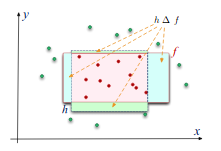
\includegraphics[scale=0.45]{./tex/induction/erm_c.png}
    \caption{Erreur entre l'hypothèse-cible et l'hypothèse apprise}
    \label{erm_c}
\end{figure}

\noindent Avec cette fonction de perte, le risque réel est égale à la probabilité qu'un exemple se situe dans la zone d'erreur entre l'hypothèse-cible et l'hypothèse apprise. En d'autres mots, il s'agit de la différence symétriques entre les deux ensembles que nous noterons $\Hat{h} \bigtriangleup h$. Une illustration de cette zone est présentée sur la Figure \ref{erm_c}.\\

\noindent Soit $\Hat{h}$ tel que $R_{reel}(\Hat{h}_S) > \epsilon$. La probabilité qu'après une observation $x \in D$, l'hypothèse apprise ne fasse pas d'erreur est donc inférieure ou égale à $1-\epsilon$.

$$P_D(\Hat{h}) = P_{(x,y) \sim D}(\Hat{h}(x)=y)$$

\noindent Supposons  m  observations:

\begin{align*}
P_D^m(\Hat{h}) &= (P_{(x,y) \sim D}(\Hat{h}(x)=y))^m\\
&\leq (1-\epsilon)^m\\
\end{align*}

\noindent Or, $1+x \leq e^x$:
$$P_D^m(\Hat{h}) \leq e^{-\epsilon m}$$

\noindent Ainsi, pour une hypothèse choisie, la probabilité de "survie est de $e^{-\epsilon m}$. Or, il est possible qu'il existe plusieurs hypothèses respectant le critère ERM mais ayant un risque réel supérieur à $\epsilon$. Ainsi, en considérant l'ensemble des hypothèses possibles $\mathcal{H}_{e}$, la probabilité qu'une hypothèse "mauvaise" soit choisie est bornée par $\sum_{h \in \mathcal{H}_\epsilon}P_D^m(\Hat{h})$

\begin{align*}
P_D^m(\forall h \in \mathcal{H}_\epsilon\Hat{h}) &= \sum_{h \in \mathcal{H}_\epsilon}P_D^m(\Hat{h})\\
&\leq |\mathcal{H}_{\epsilon}|e^{-\epsilon m}\\
&\leq |\mathcal{H}|e^{-\epsilon m}
\end{align*}

\noindent Le PAC-Learning est caractérisé par:
$$P(P_{x \sim D} (R_{reel}(\Hat{h}_S)) \leq \epsilon) > 1-\delta$$

\noindent La condition est donc respectée si:
$$m \geq \frac{1}{\epsilon}ln\frac{|\mathcal{H}|}{\delta}$$

\noindent \textbf{Important}: En réecrivant l'équation du PAC-Learning dans ce cas-ci, nous observons:
$$P(P_{x \sim D} (R_{reel}(\Hat{h}_S)) \leq \epsilon) > 1-\delta$$
$$P(P_{x \sim D} (R_{reel}(\Hat{h}_S)) \leq R_{emp}(\Hat{h})+\frac{log|\mathcal{H}|+log\frac{1}{\delta}}{m}) > 1-\delta$$

\noindent $R_{emp}(\Hat{h})=0$ par définition car nous sommes dans le cas réalisable. Nous observons donc que m est directement dépendant de $|\mathcal{H}|$ mais surtout, la borne d'erreur est directement dépendante de la cardinalité de $\mathcal{H}$. De ce fait, il est \textbf{fondamentale} de limiter l'espace des hypothèses possibles afin de favoriser l'induction. En d'autres mots, il est nécessaire de \textit{contraindre} l'espace des hypothèses avec des conditions supplémentaires. L'application de contraintes s'appelle la \textbf{Régularisation}. La \textbf{Régularisation} est très employée en Machine Learning et le Deep Learning ne fait pas exception. Elle est employée pour favoriser l'apprentissage et lutter contre le risque de sur-apprentissage.\\

\noindent \textbf{Remarque}: Cette étude de cas est relativement triviale notamment du fait qu'on a étudié le cas fini avec un espace d'hypothèse fini. Dans les cas plus généraux, l'étude de modèle est une tâche ardue et complexe qui nécessite une connaissance mathématique poussée.

\subsection{Théorie de la régularisation}
\subsubsection{Contexte et environnement}
\noindent L'induction se présente comme un problème dit \textit{mal posé}. Un problème \textit{bien posé} doit répondre à 3 critères:
\begin{itemize}
    \item \textbf{Existence}: pour toute fonction-cible h, il existe une fonction $\Hat{h} \in \mathcal{H}$ en tant que solution du problème.\\

    \item \textbf{Unicité}: $\Hat{h}$ est unique.\\

    \item \textbf{Continuité}: $\Hat{h}$ dépend \textit{continûment} de h.
\end{itemize}

\noindent Or, dans le cadre de l'induction, la condition d'unicité est souvent non respectée. De même qu'il est possible qu'il n'existe pas d'hypothèse dans $\mathcal{H}$ qui puisse parfaitement s'associer aux données, notamment si les données sont bruitées ou non représentables par l'espace $\mathcal{H}$. \\

\noindent La théorie de l'apprentissage modifie le problème \textit{mal posé} que représente le problème d'induction en ajoutant des contraintes additionnelles. Ainsi, le problème à résoudre est la recherche de $\mathcal{H}$ respectant la condition du critère inductif \textit{et} une contrainte $\Phi(\mathcal{H}) \leq \alpha$. Cette contrainte représente une caractéristique connue a priori sur la solution optimale recherchée. Elle permet de compléter la discrimination des hypothèses valides et ainsi, de diminuer le nombre d'hypothèses recevables par le modèle, i.e la cardinalité de $\mathcal{H}$.\\

\noindent Intuitivement, nous voulons supprimer les classes d'hypothèses \textit{trop} complexes, i.e capable de s'accorder à tout échantillon de dimension m. Ce type d'hypothèses est souvent associé à des hypothèses polynomiales de haute dimension. En effet, plus la dimension est élevée, plus la fonction peut expliquer une information précise du comportement observé. Or, la capacité explicative peut être telle que toute fonction de la classe peut expliquer parfaitement le comportement "grossier" issu des m exemples sans pour autant être pertinente sur l'ensemble du phénomène observé. Nous sommes donc en présence de sur-apprentissage car la fonction est trop spécialisée sur l'échantillon d'apprentissage au point de ne pas conserver une capacité de généralisation.\\

\noindent Il existe deux approches pour contraindre un espace d'hypothèses:
\begin{itemize}
    \item \textbf{Approche paramétrique}: On contraint le nombre de paramètre de l'hypothèse, i.e sa dimension. Ainsi, il est possible de limiter le nombre de connexion dans le réseau de neurones.\\

    \item \textbf{Approche non paramétrique}: Cette approche ne considère pas le nombre de paramètres mais la \textit{régularité} (smoothness) de la fonction. Ainsi, ce critère favorise les hypothèses représentées par une courbe "lisse". Une illustration est visible sur la Figure \ref{reg_no_param}. Une régularisation non paramétrique va favoriser l'hypothèse représentée par la courbe verte. Par exemple, cette régularisation limitera le degrés polynomial de l'hypothèse choisie dans le cadre d'une régression car une fonction polynomiale "lisse" tend à être une fonction polynomiale de faible degrés.
\end{itemize}

\begin{figure}
    \centering
    \includegraphics[scale=0.3]{./tex/induction/Regularization.png}
    \caption{Illustration d'une régularisation non paramétrique}
    \label{reg_no_param}
\end{figure}

\subsubsection{Définition de la régularisation}

\noindent La fonctionnelle (ou fonction) de pénalisation, que nous noterons $\Phi$, définit la connaissance a priori qui caractérise les spécificités que doivent respecter les hypothèses jugées valides par le modèle. On cherche ainsi à minimiser le \textbf{risque pénalisé}:
$$R_{reg}(h) ) R_{emp}(h) + \lambda \Phi(h)$$

\noindent $\lambda$ est un paramètre qui détermine le compromis entre la fidélité aux données d'apprentissage et les caractéristiques que doit avoir l'hypothèse. Il est difficile de connaître les caractéristiques que doit avoir l'hypothèse. Afin d'assouplir la pénalisation en cas d'informations a priori "mauvaises", le critère de pénalisation est souvent ajusté. Ainsi, on fixe la fonctionnelle mais on ajuste sa pondération selon le phénomène observé de manière empirique à partir des données d'apprentissage. En faisant varier $\lambda$, on modifie la classe d'hypothèses valorisée par le modèle. Néanmoins, comme les exemples sont issus d'un sous-ensemble de la distribution de données, les hypothèses sont nécessairement \textit{optimistes} car il est plus facile de satisfaire les conditions d'un ensemble ensemble de plus faible dimension. C'est pourquoi il est apprécié de réaliser l'apprentissage d'une fonction hypothèse pour différentes classes d'hypothèse (en faisant varier $\lambda$) et d'évaluer les différentes hypothèses sur un ensemble d'exemples indépendants de l'apprentissage (et du test). Nous parlons alors d'\textit{ensemble de validation}.

\subsubsection{Les formes de la régularisation}

\noindent Il existe trois formes principales de régularisation. Ces formes sont complémentaires et peuvent être (éventuellement) cumulées selon le cas. Ainsi, nous avons:

\begin{itemize}
    \item \textbf{Régularisation des poids}: Cette approche consiste à limiter l'importance des paramètres du modèle. En effet, un paramètre à valeur élevée favorise un sur-optimisme pour une caractéristique donnée, ce qui nuit à la capacité d'adaptation globale en sur-spécialisant l'hypothèse sur un type d'exemples non représentatif de l'ensemble du phénomène.\\

    \item \textbf{Early Stopping}: Cette approche provoque un arrêt prématuré de l'apprentissage. En effet, plus le modèle converge vers un optimum local, plus l'hypothèse devient complexe. En forçant un arrêt précoce, on limite la complexité de l'hypothèse et ainsi, le risque de perte de généralisation.\\

    \item \textbf{Échantillon bruité}: Cette approche repose sur un apprentissage à partir de données \textit{bruitées}. Les données \textit{bruitées} limite le risque que le modèle se spécialise sur l'échantillon d'apprentissage en accentuant les irégularités locales. Ainsi, l'hypothèse choisie aura tendance à favoriser les régularités dites \textit{profondes} et négligera les \textit{détails}, accentués par le bruit imposé aux données.
\end{itemize}

\subsection{No Free-lunch Theorem, un fondamental théorique (et grande désillusion ?)}

\noindent \textit{No Free Lunch Theorem}\cite{nflt} est un théorème théorique \textbf{fondamental} de l'apprentissage automatique. Ce théorème démontre une limitation forte qui modère grandement l'engouement que l'on peut avoir pour un modèle d'apprentissage ou une classe d'algorithme.\\

\noindent Supposons deux algorithmes d'apprentissage $M_1$ et $M_2$ quelconques et m, nombre de données d'apprentissage. Les propositions suivantes sont vraies:
\begin{enumerate}
    \item En moyenne uniforme sur toutes les fonctions cible f dans $\mathcal{F}$:\\
    $E_{M_1}[R_{reel}|f,m]-E_{M_2}[R_{reel}|f,m]=0$\\

    \item Pour tout échantillon d'apprentissage S, en moyenne uniforme sur toutes les fonctions cible de f dans $\mathcal{F}$:\\
    $E_{M_1}[R_{reel}|f,S]-E_{M_2}[R_{reel}|f,S]=0$\\

    \item En moyenne uniforme sur toutes les distributions possibles P(f):\\
    $E_{M_1}[R_{reel}|m]-E_{M_2}[R_{reel}|m]=0$\\

    \item Pour tout échantillon d'apprentissage S, en moyenne uniforme sur toute les distribution P(f):\\
    $E_{M_1}[R_{reel}|S]-E_{M_2}[R_{reel}|S]=0$\\
\end{enumerate}

\noindent En résumé, ces propositions démontrent \textbf{qu'aucun algorithme d'optimisation numérique n'est plus efficace qu'un autre sur l'ensemble d'un espace des problèmes}. En d'autres mots, chaque algorithme d'optimisation (aussi extraordinaire soit-il selon son créateur) est aussi performant que l'algorithme de sélection aléatoire sur l'ensemble des problématiques. Celui qui sera performant sur une classe particulière de problèmes sera mauvais sur une autre, etc... Ainsi, pas de recette miracle ! Chaque problème demandera une étude de cas poussée et un algorithme sur mesure pour le résoudre. Pour illustrer, nous pouvons voir des performances possibles et impossibles de modèles d'apprentissage sur l'ensemble des fonction-cible possible. Les signes + et - correspondent à une performance respectivement supérieure et inférieure à la sélection aléatoire. 0 indique une performance équivalente au hasard.\\

\begin{figure}
    \centering
    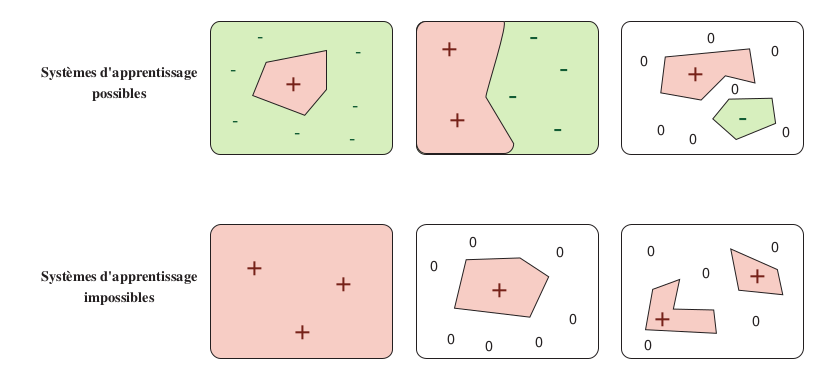
\includegraphics[scale=0.3]{./tex/induction/no_free.png}
    \caption{La fin du rêve: No Free Lunch Theorem}
    \label{no_free}
\end{figure}
\noindent Pour être capable de discriminer, un modèle repose sur des hypothèses. Ces hypothèses sont des \textbf{biais prédictifs}. Sans biais, impossible d'apprendre. Néanmoins, ces hypothèses peuvent être contre-productives pour un contexte donné et utiles dans d'autres. Il est donc nécessaire de faire des hypothèses au cas-par-cas, ce qui met fin au rêve d'un modèle parfait supérieur à tous !\\

\noindent \textbf{Remarque}: Cette restriction est néanmoins nuancée. En effet, parmi l'ensemble des problématiques de l'espace des problèmes, nombreuses sont celles qui ne correspondent pas à un phénomène réel pertinent ou "naturellement réalisable". De ce fait, il est possible de voir un modèle considéré comme "supérieur" du fait de sa grande performance sur des problématiques répandues dans notre société actuelle. Il ne faut pas oublier que cet avantage se paie dans une partie de l'espace, certes, non pertinente mais bien réelle. \\

\noindent De même, ce théorème s'applique à un modèle précis et non une classe de modèle. Dans une même classe, il existe une multitude d'architectures plus ou moins performantes selon la problématique. Dans le cadre du Deep Learning, les architectures sont particulièrement diversifiées, ce qui permet au Deep Learning d'être performant dans l'ensemble des problématiques actuelles du fait de cette richesse d'architecture. Mais il est fondamental de retenir qu'un modèle neuronal spécifique n'est pas supérieur à un autre, qu'une classe d'architecture neuronale n'est pas supérieure à une autre mais surtout, \textbf{le Deep Learning n'est pas plus performant que les architectures de Machine Learning classiques} (quoi qu'il puisse être vu, lu ou entendu...) !
